\documentclass{article}
\usepackage[margin = 0.5in]{geometry}
\usepackage{amsfonts, setspace, graphicx, amsmath, bbm, enumerate, tikz}
\graphicspath{{./images/}}

\begin{document}
    \onehalfspacing

    \begin{singlespace}
        \title{CSE 417T: Homework 4} 
        \author{Hangxiao Zhu}
        \date{\today}
        \maketitle
    \end{singlespace}

    \section*{Problem 1.}
    Results: \\
    For each of the binary classification problems, graphically report the training set error and the test 
    set error as a function of the number of weak hypotheses.
    \begin{figure}[!htb]
        \begin{center}
            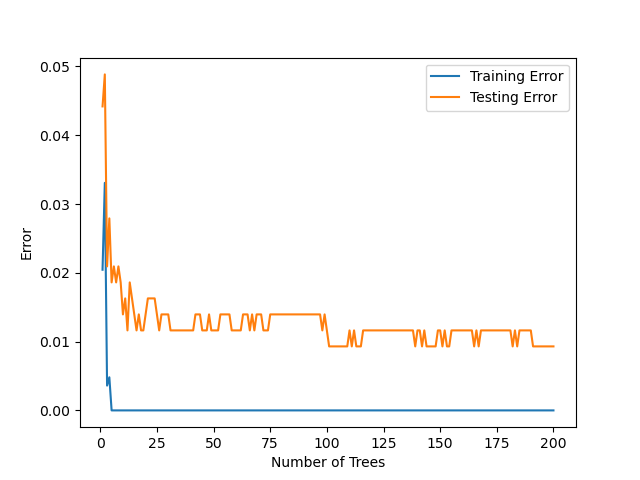
\includegraphics[width=9.6cm, height=7.2cm]{one_three.png}
            \textbf{\caption{``1-vs-3'' Problem}}
        \end{center}
    \end{figure}
    \begin{figure}[!htb]
    \begin{center}
        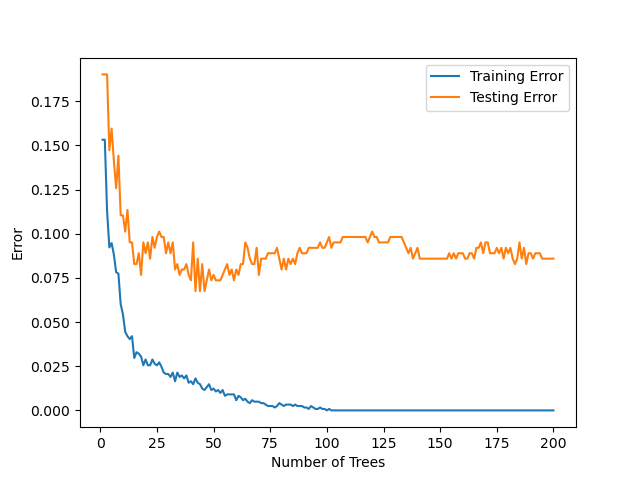
\includegraphics[width=9.6cm, height=7.2cm]{three_five.png}
        \textbf{\caption{``3-vs-5'' Problem}}
    \end{center}
    \end{figure}\\
    For each of the binary classification problems, report the final training set error and test set error.
    \begin{center}
        \begin{tabular}{|c|c|c|}
            \hline
            & Training error & Test error\\
            \hline
            ``1-vs-3'' Problem & 0.0 & 0.009302325581395349\\
            \hline
            ``3-vs-5'' Problem & 0.0 & 0.08588957055214724\\
            \hline
        \end{tabular}
    \end{center}
    Summary and interpretation of the results:
    \begin{itemize}
        \item Compare the test error of AdaBoost to the test error of Bagging, it's clear that AdaBoost
        performs better.
        \item As the number of weak hypotheses increases, both the training and test error decrease.
        \item According to the test erros to each problem, AdaBoost performs better on ``1-vs-3'' Problem. I think
        it's because 1 and 3 have more distinct characteristic differences, such as symmetries.
        \item According to the curves, AdaBoost shows robustness to overfitting. I think it's because we used
        the very simple weak learner 'decision stumps'. However, for ``3-vs-5'' Problem, AdaBoost shows signs of 
        overfitting. I think it's because the data of number 5 is more noisy.
    \end{itemize}

    \newpage
    \section*{Problem 2.}
    With the test example $x = 3.2$, we can its determine the 3 nearest neighbors are 
    $(3, 5)$, $(2,11)$, $(3,8)$. Therefore we can predict this test example's $y$ value as:
    \begin{align*}
        g(x) &= \frac{1}{k} \sum_{i = 1}^{k}y_{[i]}(x)\\
        &= \frac{1}{3} \sum_{i = 1}^{3}y_{[i]}(3.2)\\
        &= \frac{1}{3} (5 + 11 + 8)\\
        &= 8
    \end{align*}
    Therefore, I would predict $y = 8$ for this test example.

    \newpage
    \section*{Problem 3.}
    First, we map the input $(x_1, x_2)$ into the space consisting of $x_1$ and $x_1x_2$.
    \begin{center}
        \begin{tabular}{|c|c|c|c|c|}
            \hline
            & $x_1$ & $x_2$ & $x_1$ & $x_1x_2$\\
            \hline
            A & 1 & 1 & 1 & 1\\
            \hline
            B & 1 & -1 & 1 & -1\\
            \hline
            C & -1 & 1 & -1 & -1\\
            \hline
            D & -1 & -1 & -1 & 1\\
            \hline
        \end{tabular}
    \end{center}
    We know points A and D should be labeled as -1, and points B and C should be labeled as +1.\\
    Then, we draw the four input points in this space with the maximal margin separator. The maximal margin 
    separator is the line $x_1x_2 = 0$ and the margin is 1.
    \begin{center}
        \begin{tikzpicture}
            \draw[->] (-3.2,0)--(3.2,0) node[right] {$x_1$};
            \draw[->] (0,-3.2)--(0,3.2) node[right] {$x_1x_2$};
            \foreach \x in {0,1,...,4}
            {
                \draw[xshift=\x cm] (-2,0) -- (-2,0.1);
                \draw[yshift=\x cm] (0,-2) -- (0.1,-2);
            };

            \node[below] at (0.2,0){0};
            \foreach \x in {-2,...,-1}
                \node[below] at(\x,0){\x};
            \foreach \y in {1,...,2}
                \node[below] at(\y,0){\y};
            \foreach \y in {-2,...,-1}
                \node[left] at(0,\y){\y};
            \foreach \y in {1,...,2}
                \node[left] at(0,\y){\y};

            \foreach \Point/\PointLabel in {(1,1)/A, (1,-1)/B, (-1,-1)/C, (-1,1)/D}{
                \draw[fill=black] \Point circle (0.05) node[above right] {$\PointLabel$};
            }

            \draw[red, very thick] (-3,0) -- (3,0);
        \end{tikzpicture}
    \end{center}
    Now, we draw the four input points back in the original Euclidean input space with the separating line.
    \begin{center}
        \begin{tikzpicture}
            \draw[->] (-3.2,0)--(3.2,0) node[right] {$x_1$};
            \draw[->] (0,-3.2)--(0,3.2) node[right] {$x_2$};
            \foreach \x in {0,1,...,4}
            {
                \draw[xshift=\x cm] (-2,0) -- (-2,0.1);
                \draw[yshift=\x cm] (0,-2) -- (0.1,-2);
            };

            \node[below] at (0.2,0){0};
            \foreach \x in {-2,...,-1}
                \node[below] at(\x,0){\x};
            \foreach \y in {1,...,2}
                \node[below] at(\y,0){\y};
            \foreach \y in {-2,...,-1}
                \node[left] at(0,\y){\y};
            \foreach \y in {1,...,2}
                \node[left] at(0,\y){\y};

            \foreach \Point/\PointLabel in {(1,1)/A, (1,-1)/B, (-1,1)/C, (-1,-1)/D}{
                \draw[fill=black] \Point circle (0.05) node[above right] {$\PointLabel$};
            }

            \draw[red, very thick] (-3,0) -- (0,0) -- (0,3);
            \draw[blue, very thick] (0,-3) -- (0,0) -- (3,0);
        \end{tikzpicture}
    \end{center}

    \newpage
    \section*{Problem 4.}
    First, we denote the squared Euclidean distance of the two points $\Phi(\overset{\to}{x_i})$ and 
    $\Phi(\overset{\to}{x_j})$ as $sd_E$. And we assume each $\Phi(\overset{\to}{x})$ has a dimension 
    of $n$.\\
    We can deduce that 
    \begin{align*}
        sd_E &= \sum_{k = 1}^{n} (\Phi(\overset{\to}{x_i})_k - \Phi(\overset{\to}{x_j})_k)^2\\
        &= \sum_{k = 1}^{n} (\Phi(\overset{\to}{x_i})_k)^2 + \sum_{k = 1}^{n} (\Phi(\overset{\to}{x_j})_k)^2
        - \sum_{k = 1}^{n} 2 \Phi(\overset{\to}{x_i})_k \Phi(\overset{\to}{x_j})_k\\
        &= \Phi(\overset{\to}{x_i})^T \Phi(\overset{\to}{x_i}) + 
        \Phi(\overset{\to}{x_j})^T \Phi(\overset{\to}{x_j}) - 
        2\Phi(\overset{\to}{x_i})^T \Phi(\overset{\to}{x_j})
    \end{align*}
    Since we have the kernel function
    \begin{align*}
        K(\overset{\to}{x_i}, \overset{\to}{x_j}) &= \Phi(\overset{\to}{x_i})^T \Phi(\overset{\to}{x_j})
    \end{align*}
    We can write down the squared Euclidean distance using the kernel function K as
    \begin{align*}
        sd_E &= K(\overset{\to}{x_i}, \overset{\to}{x_i}) + K(\overset{\to}{x_j}, \overset{\to}{x_j})
        - 2K(\overset{\to}{x_i}, \overset{\to}{x_j})
    \end{align*}

    \newpage
    \section*{Problem 5.}
    First, we simplify the Boolean formula.
    \begin{align*}
        XOR(AND(x_1, x_2), x_3) &= (x_1 \wedge x_2) \oplus x_3\\
        &= ((x_1 \wedge x_2) \wedge \urcorner x_3) \vee (\urcorner(x_1 \wedge x_2) \wedge x_3)\\
        &= (x_1 \wedge x_2 \wedge \urcorner x_3) \vee ((\urcorner x_1 \vee \urcorner x_2) \wedge x_3)\\
        &= (x_1 \wedge x_2 \wedge \urcorner x_3) \vee (\urcorner x_1 \wedge x_3) \vee 
        (\urcorner x_2 \wedge x_3)\\
    \end{align*}
    Then, design the neural network.
    \begin{figure}[!htb]
        \begin{center}
            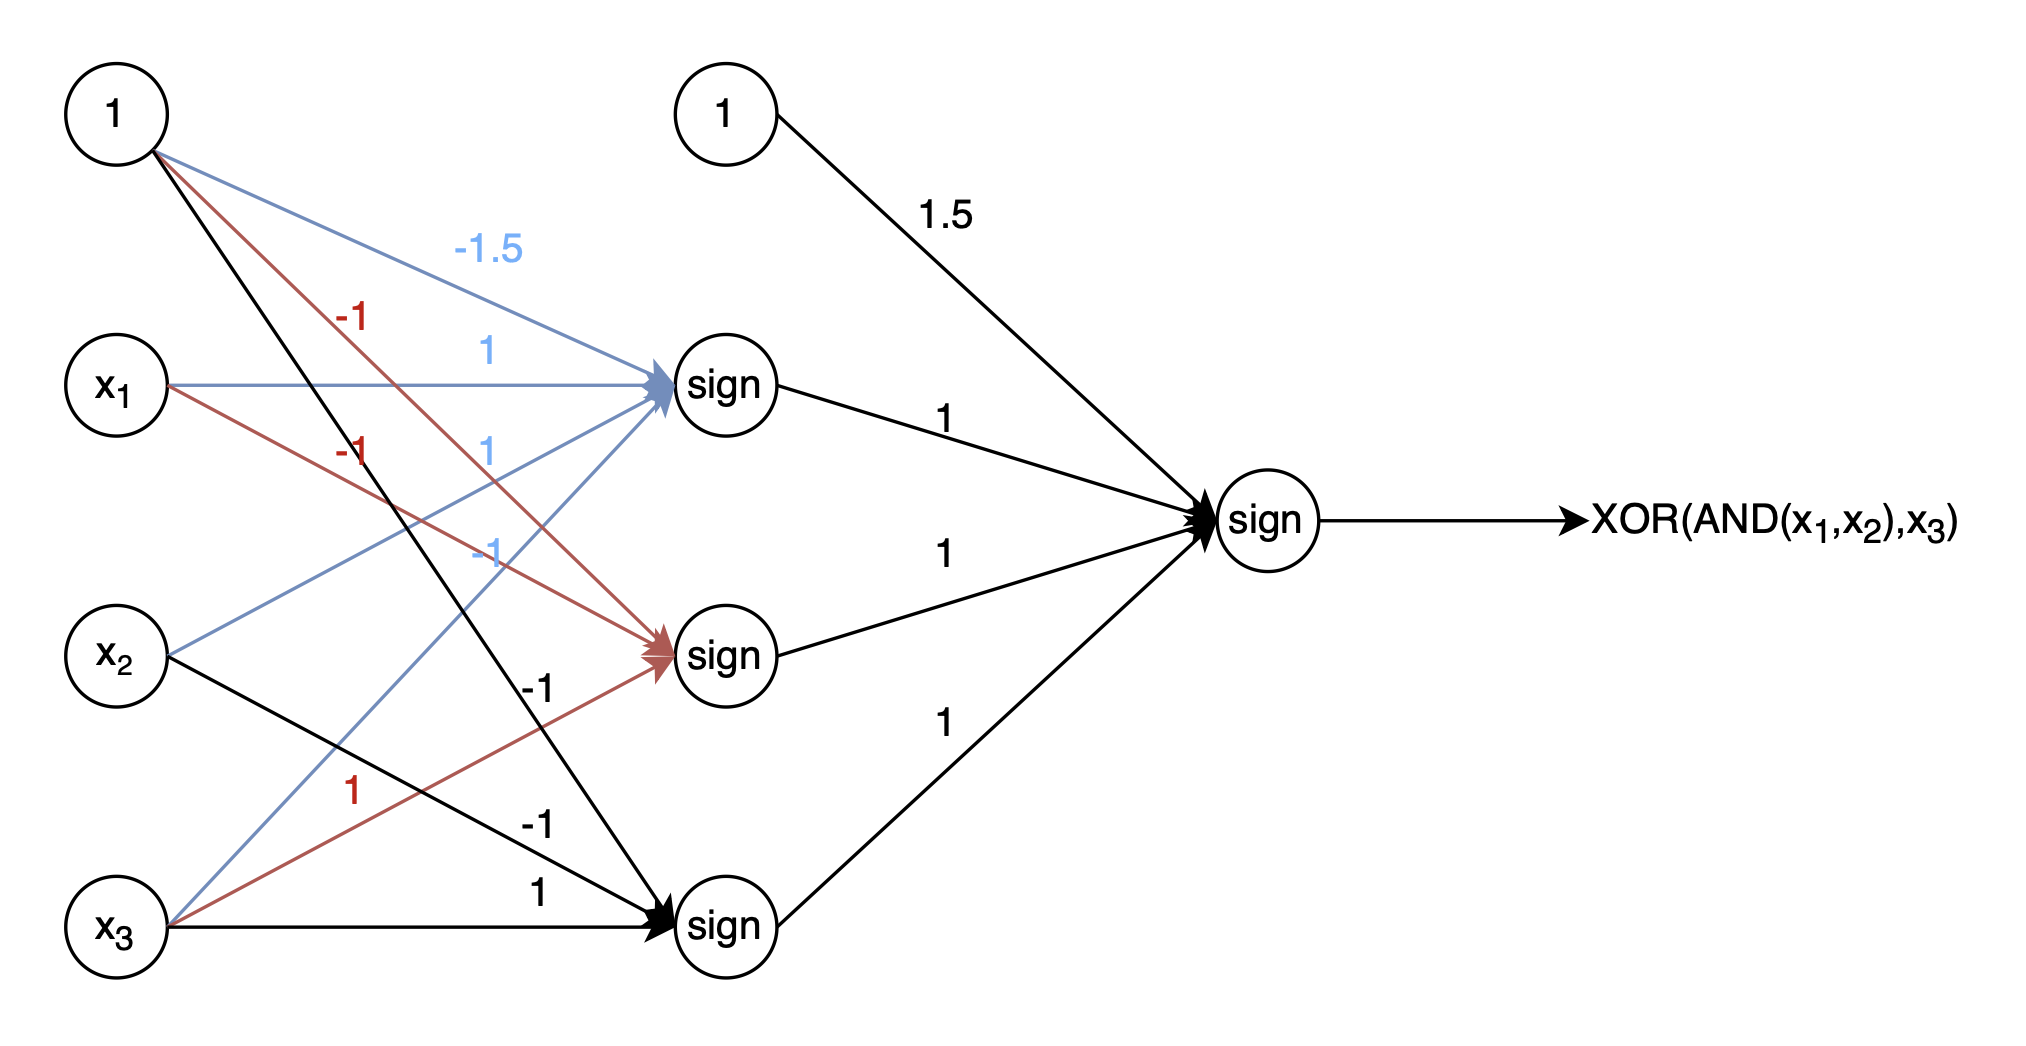
\includegraphics[width=10.13cm, height=5.23cm]{nn.png}x
            \textbf{\caption{Neural Network for XOR(AND($x_1$, $x_2$), $x_3$)}}
        \end{center}
    \end{figure}

    \newpage
    \section*{Problem 6.}
    a. Given that 
    \begin{align*}
        \text{tanh}(s) &= \frac{e^s - e^{-s}}{e^s + e^{-s}}\\
        \text{tanh}'(s) &= 1 - \text{tanh}^2(s)
    \end{align*}
    We have
    \begin{align*}
        \nabla \mathbb{E}_{in}(\overset{\to}{w}) &= 
        \nabla \frac{1}{N} \sum_{n = 1}^{N} (\text{tanh}(\overset{\to}{w}^T \overset{\to}{x}_n) - y_n)^2\\
        &= \frac{1}{N} \sum_{n = 1}^{N} 2 (\text{tanh}(\overset{\to}{w}^T \overset{\to}{x}_n) - y_n)
        (\frac{\mathrm{d} \text{tanh}(\overset{\to}{w}^T \overset{\to}{x}_n)}
        {\mathrm{d} \overset{\to}{w}})\\
        &= \frac{1}{N} \sum_{n = 1}^{N} 2 (\text{tanh}(\overset{\to}{w}^T \overset{\to}{x}_n) - y_n)
        (1 - \text{tanh}^2(\overset{\to}{w}^T \overset{\to}{x}_n)) \overset{\to}{x}_n\\
        &= \frac{2}{N} \sum_{n = 1}^{N} (\text{tanh}(\overset{\to}{w}^T \overset{\to}{x}_n) - y_n)
        (1 - \text{tanh}^2(\overset{\to}{w}^T \overset{\to}{x}_n)) \overset{\to}{x}_n
    \end{align*}
    Based on this equation, when $\overset{\to}{w}$ consists large weights, that $\overset{\to}{w} \to \infty$, 
    $\text{tanh}(\overset{\to}{w}) \to 1$, $\nabla \mathbb{E}_{in}(\overset{\to}{w}) \to 0$. That means with large 
    weights, the gradient will not change, thus the hypothesis will not be improved.\\
    Based on the conclusion above, when using gradient descent to optimize the weights of a sigmoidal perceptron, 
    it is not a good idea to initialize the weights to be very, very large.\\
    b. If all the weights are set to zero, then each output from the input layer will be zero. That means each 
    $y_n = \overset{\to}{w}^T \overset{\to}{x}_n = 0$, and $\text{tanh}(\overset{\to}{w}^T \overset{\to}{x}_n) = 0$.
    Based on the equation in question a, we know $\nabla \mathbb{E}_{in}(\overset{\to}{w}) = 0$. Thus, when we use
    gradient descent to update weights, weights will remain zero. Therefore, it is not a good idea to initialize the 
    weights to zero.

\end{document}